% Created by tikzDevice version 0.10.1 on 2017-11-06 20:32:22
% !TEX encoding = UTF-8 Unicode
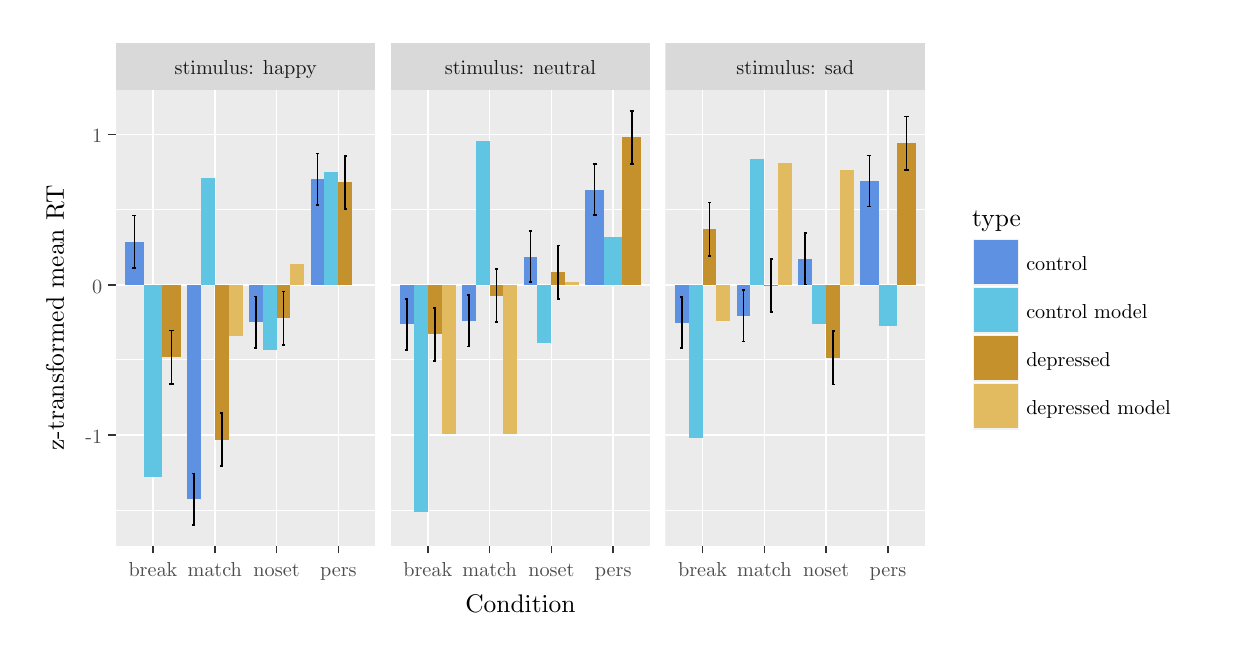
\begin{tikzpicture}[x=1pt,y=1pt]
\definecolor{fillColor}{RGB}{255,255,255}
\path[use as bounding box,fill=fillColor,fill opacity=0.00] (0,0) rectangle (433.62,216.81);
\begin{scope}
\path[clip] (  0.00,  0.00) rectangle (433.62,216.81);
\definecolor{drawColor}{RGB}{255,255,255}
\definecolor{fillColor}{RGB}{255,255,255}

\path[draw=drawColor,line width= 0.6pt,line join=round,line cap=round,fill=fillColor] (  0.00,  0.00) rectangle (433.62,216.81);
\end{scope}
\begin{scope}
\path[clip] ( 31.87, 29.59) rectangle (125.67,194.25);
\definecolor{fillColor}{gray}{0.92}

\path[fill=fillColor] ( 31.87, 29.59) rectangle (125.67,194.25);
\definecolor{drawColor}{RGB}{255,255,255}

\path[draw=drawColor,line width= 0.3pt,line join=round] ( 31.87, 42.48) --
	(125.67, 42.48);

\path[draw=drawColor,line width= 0.3pt,line join=round] ( 31.87, 96.76) --
	(125.67, 96.76);

\path[draw=drawColor,line width= 0.3pt,line join=round] ( 31.87,151.03) --
	(125.67,151.03);

\path[draw=drawColor,line width= 0.6pt,line join=round] ( 31.87, 69.62) --
	(125.67, 69.62);

\path[draw=drawColor,line width= 0.6pt,line join=round] ( 31.87,123.90) --
	(125.67,123.90);

\path[draw=drawColor,line width= 0.6pt,line join=round] ( 31.87,178.17) --
	(125.67,178.17);

\path[draw=drawColor,line width= 0.6pt,line join=round] ( 45.27, 29.59) --
	( 45.27,194.25);

\path[draw=drawColor,line width= 0.6pt,line join=round] ( 67.60, 29.59) --
	( 67.60,194.25);

\path[draw=drawColor,line width= 0.6pt,line join=round] ( 89.93, 29.59) --
	( 89.93,194.25);

\path[draw=drawColor,line width= 0.6pt,line join=round] (112.27, 29.59) --
	(112.27,194.25);
\definecolor{fillColor}{RGB}{196,145,45}

\path[fill=fillColor] ( 48.62, 97.73) rectangle ( 55.32,123.90);
\definecolor{fillColor}{RGB}{95,197,226}

\path[fill=fillColor] ( 41.92, 54.35) rectangle ( 48.62,123.90);
\definecolor{fillColor}{RGB}{95,145,226}

\path[fill=fillColor] ( 35.22,123.90) rectangle ( 41.92,139.47);
\definecolor{fillColor}{RGB}{226,186,95}

\path[fill=fillColor] ( 72.63,105.40) rectangle ( 77.65,123.90);
\definecolor{fillColor}{RGB}{196,145,45}

\path[fill=fillColor] ( 67.60, 67.99) rectangle ( 72.63,123.90);
\definecolor{fillColor}{RGB}{95,197,226}

\path[fill=fillColor] ( 62.58,123.90) rectangle ( 67.60,162.58);
\definecolor{fillColor}{RGB}{95,145,226}

\path[fill=fillColor] ( 57.55, 46.37) rectangle ( 62.58,123.90);
\definecolor{fillColor}{RGB}{226,186,95}

\path[fill=fillColor] ( 94.96,123.90) rectangle ( 99.98,131.34);
\definecolor{fillColor}{RGB}{196,145,45}

\path[fill=fillColor] ( 89.93,111.83) rectangle ( 94.96,123.90);
\definecolor{fillColor}{RGB}{95,197,226}

\path[fill=fillColor] ( 84.91,100.42) rectangle ( 89.93,123.90);
\definecolor{fillColor}{RGB}{95,145,226}

\path[fill=fillColor] ( 79.88,110.41) rectangle ( 84.91,123.90);
\definecolor{fillColor}{RGB}{196,145,45}

\path[fill=fillColor] (112.27,123.90) rectangle (117.29,160.90);
\definecolor{fillColor}{RGB}{95,197,226}

\path[fill=fillColor] (107.24,123.90) rectangle (112.27,164.69);
\definecolor{fillColor}{RGB}{95,145,226}

\path[fill=fillColor] (102.22,123.90) rectangle (107.24,162.07);
\definecolor{drawColor}{RGB}{0,0,0}

\path[draw=drawColor,line width= 0.6pt,line join=round] ( 51.23,107.36) --
	( 52.71,107.36);

\path[draw=drawColor,line width= 0.6pt,line join=round] ( 51.97,107.36) --
	( 51.97, 88.09);

\path[draw=drawColor,line width= 0.6pt,line join=round] ( 51.23, 88.09) --
	( 52.71, 88.09);

\path[draw=drawColor,line width= 0.6pt,line join=round] ( 37.83,148.99) --
	( 39.32,148.99);

\path[draw=drawColor,line width= 0.6pt,line join=round] ( 38.57,148.99) --
	( 38.57,129.96);

\path[draw=drawColor,line width= 0.6pt,line join=round] ( 37.83,129.96) --
	( 39.32,129.96);

\path[draw=drawColor,line width= 0.6pt,line join=round] ( 69.56, 77.59) --
	( 70.67, 77.59);

\path[draw=drawColor,line width= 0.6pt,line join=round] ( 70.11, 77.59) --
	( 70.11, 58.38);

\path[draw=drawColor,line width= 0.6pt,line join=round] ( 69.56, 58.38) --
	( 70.67, 58.38);

\path[draw=drawColor,line width= 0.6pt,line join=round] ( 59.51, 55.67) --
	( 60.62, 55.67);

\path[draw=drawColor,line width= 0.6pt,line join=round] ( 60.07, 55.67) --
	( 60.07, 37.07);

\path[draw=drawColor,line width= 0.6pt,line join=round] ( 59.51, 37.07) --
	( 60.62, 37.07);

\path[draw=drawColor,line width= 0.6pt,line join=round] ( 91.89,121.43) --
	( 93.00,121.43);

\path[draw=drawColor,line width= 0.6pt,line join=round] ( 92.45,121.43) --
	( 92.45,102.22);

\path[draw=drawColor,line width= 0.6pt,line join=round] ( 91.89,102.22) --
	( 93.00,102.22);

\path[draw=drawColor,line width= 0.6pt,line join=round] ( 81.84,119.71) --
	( 82.96,119.71);

\path[draw=drawColor,line width= 0.6pt,line join=round] ( 82.40,119.71) --
	( 82.40,101.11);

\path[draw=drawColor,line width= 0.6pt,line join=round] ( 81.84,101.11) --
	( 82.96,101.11);

\path[draw=drawColor,line width= 0.6pt,line join=round] (114.22,170.51) --
	(115.34,170.51);

\path[draw=drawColor,line width= 0.6pt,line join=round] (114.78,170.51) --
	(114.78,151.30);

\path[draw=drawColor,line width= 0.6pt,line join=round] (114.22,151.30) --
	(115.34,151.30);

\path[draw=drawColor,line width= 0.6pt,line join=round] (104.17,171.34) --
	(105.29,171.34);

\path[draw=drawColor,line width= 0.6pt,line join=round] (104.73,171.34) --
	(104.73,152.80);

\path[draw=drawColor,line width= 0.6pt,line join=round] (104.17,152.80) --
	(105.29,152.80);
\end{scope}
\begin{scope}
\path[clip] (131.17, 29.59) rectangle (224.96,194.25);
\definecolor{fillColor}{gray}{0.92}

\path[fill=fillColor] (131.17, 29.59) rectangle (224.96,194.25);
\definecolor{drawColor}{RGB}{255,255,255}

\path[draw=drawColor,line width= 0.3pt,line join=round] (131.17, 42.48) --
	(224.96, 42.48);

\path[draw=drawColor,line width= 0.3pt,line join=round] (131.17, 96.76) --
	(224.96, 96.76);

\path[draw=drawColor,line width= 0.3pt,line join=round] (131.17,151.03) --
	(224.96,151.03);

\path[draw=drawColor,line width= 0.6pt,line join=round] (131.17, 69.62) --
	(224.96, 69.62);

\path[draw=drawColor,line width= 0.6pt,line join=round] (131.17,123.90) --
	(224.96,123.90);

\path[draw=drawColor,line width= 0.6pt,line join=round] (131.17,178.17) --
	(224.96,178.17);

\path[draw=drawColor,line width= 0.6pt,line join=round] (144.56, 29.59) --
	(144.56,194.25);

\path[draw=drawColor,line width= 0.6pt,line join=round] (166.90, 29.59) --
	(166.90,194.25);

\path[draw=drawColor,line width= 0.6pt,line join=round] (189.23, 29.59) --
	(189.23,194.25);

\path[draw=drawColor,line width= 0.6pt,line join=round] (211.56, 29.59) --
	(211.56,194.25);
\definecolor{fillColor}{RGB}{226,186,95}

\path[fill=fillColor] (149.59, 69.89) rectangle (154.61,123.90);
\definecolor{fillColor}{RGB}{196,145,45}

\path[fill=fillColor] (144.56,105.98) rectangle (149.59,123.90);
\definecolor{fillColor}{RGB}{95,197,226}

\path[fill=fillColor] (139.54, 41.82) rectangle (144.56,123.90);
\definecolor{fillColor}{RGB}{95,145,226}

\path[fill=fillColor] (134.51,109.61) rectangle (139.54,123.90);
\definecolor{fillColor}{RGB}{226,186,95}

\path[fill=fillColor] (171.92, 69.84) rectangle (176.95,123.90);
\definecolor{fillColor}{RGB}{196,145,45}

\path[fill=fillColor] (166.90,119.96) rectangle (171.92,123.90);
\definecolor{fillColor}{RGB}{95,197,226}

\path[fill=fillColor] (161.87,123.90) rectangle (166.90,175.84);
\definecolor{fillColor}{RGB}{95,145,226}

\path[fill=fillColor] (156.85,110.90) rectangle (161.87,123.90);
\definecolor{fillColor}{RGB}{226,186,95}

\path[fill=fillColor] (194.25,123.90) rectangle (199.28,124.87);
\definecolor{fillColor}{RGB}{196,145,45}

\path[fill=fillColor] (189.23,123.90) rectangle (194.25,128.45);
\definecolor{fillColor}{RGB}{95,197,226}

\path[fill=fillColor] (184.20,102.85) rectangle (189.23,123.90);
\definecolor{fillColor}{RGB}{95,145,226}

\path[fill=fillColor] (179.18,123.90) rectangle (184.20,134.12);
\definecolor{fillColor}{RGB}{196,145,45}

\path[fill=fillColor] (214.91,123.90) rectangle (221.61,177.16);
\definecolor{fillColor}{RGB}{95,197,226}

\path[fill=fillColor] (208.21,123.90) rectangle (214.91,141.08);
\definecolor{fillColor}{RGB}{95,145,226}

\path[fill=fillColor] (201.51,123.90) rectangle (208.21,158.32);
\definecolor{drawColor}{RGB}{0,0,0}

\path[draw=drawColor,line width= 0.6pt,line join=round] (146.52,115.58) --
	(147.63,115.58);

\path[draw=drawColor,line width= 0.6pt,line join=round] (147.08,115.58) --
	(147.08, 96.37);

\path[draw=drawColor,line width= 0.6pt,line join=round] (146.52, 96.37) --
	(147.63, 96.37);

\path[draw=drawColor,line width= 0.6pt,line join=round] (136.47,118.88) --
	(137.59,118.88);

\path[draw=drawColor,line width= 0.6pt,line join=round] (137.03,118.88) --
	(137.03,100.34);

\path[draw=drawColor,line width= 0.6pt,line join=round] (136.47,100.34) --
	(137.59,100.34);

\path[draw=drawColor,line width= 0.6pt,line join=round] (168.85,129.56) --
	(169.97,129.56);

\path[draw=drawColor,line width= 0.6pt,line join=round] (169.41,129.56) --
	(169.41,110.35);

\path[draw=drawColor,line width= 0.6pt,line join=round] (168.85,110.35) --
	(169.97,110.35);

\path[draw=drawColor,line width= 0.6pt,line join=round] (158.80,120.17) --
	(159.92,120.17);

\path[draw=drawColor,line width= 0.6pt,line join=round] (159.36,120.17) --
	(159.36,101.64);

\path[draw=drawColor,line width= 0.6pt,line join=round] (158.80,101.64) --
	(159.92,101.64);

\path[draw=drawColor,line width= 0.6pt,line join=round] (191.18,138.09) --
	(192.30,138.09);

\path[draw=drawColor,line width= 0.6pt,line join=round] (191.74,138.09) --
	(191.74,118.82);

\path[draw=drawColor,line width= 0.6pt,line join=round] (191.18,118.82) --
	(192.30,118.82);

\path[draw=drawColor,line width= 0.6pt,line join=round] (181.13,143.39) --
	(182.25,143.39);

\path[draw=drawColor,line width= 0.6pt,line join=round] (181.69,143.39) --
	(181.69,124.85);

\path[draw=drawColor,line width= 0.6pt,line join=round] (181.13,124.85) --
	(182.25,124.85);

\path[draw=drawColor,line width= 0.6pt,line join=round] (217.52,186.76) --
	(219.00,186.76);

\path[draw=drawColor,line width= 0.6pt,line join=round] (218.26,186.76) --
	(218.26,167.55);

\path[draw=drawColor,line width= 0.6pt,line join=round] (217.52,167.55) --
	(219.00,167.55);

\path[draw=drawColor,line width= 0.6pt,line join=round] (204.12,167.58) --
	(205.60,167.58);

\path[draw=drawColor,line width= 0.6pt,line join=round] (204.86,167.58) --
	(204.86,149.05);

\path[draw=drawColor,line width= 0.6pt,line join=round] (204.12,149.05) --
	(205.60,149.05);
\end{scope}
\begin{scope}
\path[clip] (230.46, 29.59) rectangle (324.25,194.25);
\definecolor{fillColor}{gray}{0.92}

\path[fill=fillColor] (230.46, 29.59) rectangle (324.25,194.25);
\definecolor{drawColor}{RGB}{255,255,255}

\path[draw=drawColor,line width= 0.3pt,line join=round] (230.46, 42.48) --
	(324.25, 42.48);

\path[draw=drawColor,line width= 0.3pt,line join=round] (230.46, 96.76) --
	(324.25, 96.76);

\path[draw=drawColor,line width= 0.3pt,line join=round] (230.46,151.03) --
	(324.25,151.03);

\path[draw=drawColor,line width= 0.6pt,line join=round] (230.46, 69.62) --
	(324.25, 69.62);

\path[draw=drawColor,line width= 0.6pt,line join=round] (230.46,123.90) --
	(324.25,123.90);

\path[draw=drawColor,line width= 0.6pt,line join=round] (230.46,178.17) --
	(324.25,178.17);

\path[draw=drawColor,line width= 0.6pt,line join=round] (243.86, 29.59) --
	(243.86,194.25);

\path[draw=drawColor,line width= 0.6pt,line join=round] (266.19, 29.59) --
	(266.19,194.25);

\path[draw=drawColor,line width= 0.6pt,line join=round] (288.52, 29.59) --
	(288.52,194.25);

\path[draw=drawColor,line width= 0.6pt,line join=round] (310.85, 29.59) --
	(310.85,194.25);
\definecolor{fillColor}{RGB}{226,186,95}

\path[fill=fillColor] (248.88,110.83) rectangle (253.91,123.90);
\definecolor{fillColor}{RGB}{196,145,45}

\path[fill=fillColor] (243.86,123.90) rectangle (248.88,144.03);
\definecolor{fillColor}{RGB}{95,197,226}

\path[fill=fillColor] (238.83, 68.58) rectangle (243.86,123.90);
\definecolor{fillColor}{RGB}{95,145,226}

\path[fill=fillColor] (233.81,110.23) rectangle (238.83,123.90);
\definecolor{fillColor}{RGB}{226,186,95}

\path[fill=fillColor] (271.21,123.90) rectangle (276.24,167.78);
\definecolor{fillColor}{RGB}{196,145,45}

\path[fill=fillColor] (266.19,123.71) rectangle (271.21,123.90);
\definecolor{fillColor}{RGB}{95,197,226}

\path[fill=fillColor] (261.17,123.90) rectangle (266.19,169.40);
\definecolor{fillColor}{RGB}{95,145,226}

\path[fill=fillColor] (256.14,112.69) rectangle (261.17,123.90);
\definecolor{fillColor}{RGB}{226,186,95}

\path[fill=fillColor] (293.55,123.90) rectangle (298.57,165.52);
\definecolor{fillColor}{RGB}{196,145,45}

\path[fill=fillColor] (288.52, 97.54) rectangle (293.55,123.90);
\definecolor{fillColor}{RGB}{95,197,226}

\path[fill=fillColor] (283.50,109.71) rectangle (288.52,123.90);
\definecolor{fillColor}{RGB}{95,145,226}

\path[fill=fillColor] (278.47,123.90) rectangle (283.50,133.32);
\definecolor{fillColor}{RGB}{196,145,45}

\path[fill=fillColor] (314.20,123.90) rectangle (320.90,175.07);
\definecolor{fillColor}{RGB}{95,197,226}

\path[fill=fillColor] (307.50,109.12) rectangle (314.20,123.90);
\definecolor{fillColor}{RGB}{95,145,226}

\path[fill=fillColor] (300.80,123.90) rectangle (307.50,161.39);
\definecolor{drawColor}{RGB}{0,0,0}

\path[draw=drawColor,line width= 0.6pt,line join=round] (245.81,153.67) --
	(246.93,153.67);

\path[draw=drawColor,line width= 0.6pt,line join=round] (246.37,153.67) --
	(246.37,134.40);

\path[draw=drawColor,line width= 0.6pt,line join=round] (245.81,134.40) --
	(246.93,134.40);

\path[draw=drawColor,line width= 0.6pt,line join=round] (235.76,119.50) --
	(236.88,119.50);

\path[draw=drawColor,line width= 0.6pt,line join=round] (236.32,119.50) --
	(236.32,100.96);

\path[draw=drawColor,line width= 0.6pt,line join=round] (235.76,100.96) --
	(236.88,100.96);

\path[draw=drawColor,line width= 0.6pt,line join=round] (268.14,133.31) --
	(269.26,133.31);

\path[draw=drawColor,line width= 0.6pt,line join=round] (268.70,133.31) --
	(268.70,114.10);

\path[draw=drawColor,line width= 0.6pt,line join=round] (268.14,114.10) --
	(269.26,114.10);

\path[draw=drawColor,line width= 0.6pt,line join=round] (258.09,121.96) --
	(259.21,121.96);

\path[draw=drawColor,line width= 0.6pt,line join=round] (258.65,121.96) --
	(258.65,103.42);

\path[draw=drawColor,line width= 0.6pt,line join=round] (258.09,103.42) --
	(259.21,103.42);

\path[draw=drawColor,line width= 0.6pt,line join=round] (290.48,107.15) --
	(291.59,107.15);

\path[draw=drawColor,line width= 0.6pt,line join=round] (291.03,107.15) --
	(291.03, 87.93);

\path[draw=drawColor,line width= 0.6pt,line join=round] (290.48, 87.93) --
	(291.59, 87.93);

\path[draw=drawColor,line width= 0.6pt,line join=round] (280.43,142.58) --
	(281.54,142.58);

\path[draw=drawColor,line width= 0.6pt,line join=round] (280.98,142.58) --
	(280.98,124.05);

\path[draw=drawColor,line width= 0.6pt,line join=round] (280.43,124.05) --
	(281.54,124.05);

\path[draw=drawColor,line width= 0.6pt,line join=round] (316.81,184.67) --
	(318.30,184.67);

\path[draw=drawColor,line width= 0.6pt,line join=round] (317.55,184.67) --
	(317.55,165.46);

\path[draw=drawColor,line width= 0.6pt,line join=round] (316.81,165.46) --
	(318.30,165.46);

\path[draw=drawColor,line width= 0.6pt,line join=round] (303.41,170.66) --
	(304.90,170.66);

\path[draw=drawColor,line width= 0.6pt,line join=round] (304.15,170.66) --
	(304.15,152.13);

\path[draw=drawColor,line width= 0.6pt,line join=round] (303.41,152.13) --
	(304.90,152.13);
\end{scope}
\begin{scope}
\path[clip] ( 31.87,194.25) rectangle (125.67,211.31);
\definecolor{fillColor}{gray}{0.85}

\path[fill=fillColor] ( 31.87,194.25) rectangle (125.67,211.31);
\definecolor{drawColor}{gray}{0.10}

\node[text=drawColor,anchor=base,inner sep=0pt, outer sep=0pt, scale=  0.73] at ( 78.77,199.75) {stimulus: happy};
\end{scope}
\begin{scope}
\path[clip] (131.17,194.25) rectangle (224.96,211.31);
\definecolor{fillColor}{gray}{0.85}

\path[fill=fillColor] (131.17,194.25) rectangle (224.96,211.31);
\definecolor{drawColor}{gray}{0.10}

\node[text=drawColor,anchor=base,inner sep=0pt, outer sep=0pt, scale=  0.73] at (178.06,199.75) {stimulus: neutral};
\end{scope}
\begin{scope}
\path[clip] (230.46,194.25) rectangle (324.25,211.31);
\definecolor{fillColor}{gray}{0.85}

\path[fill=fillColor] (230.46,194.25) rectangle (324.25,211.31);
\definecolor{drawColor}{gray}{0.10}

\node[text=drawColor,anchor=base,inner sep=0pt, outer sep=0pt, scale=  0.73] at (277.36,199.75) {stimulus: sad};
\end{scope}
\begin{scope}
\path[clip] (  0.00,  0.00) rectangle (433.62,216.81);
\definecolor{drawColor}{gray}{0.20}

\path[draw=drawColor,line width= 0.6pt,line join=round] ( 45.27, 26.84) --
	( 45.27, 29.59);

\path[draw=drawColor,line width= 0.6pt,line join=round] ( 67.60, 26.84) --
	( 67.60, 29.59);

\path[draw=drawColor,line width= 0.6pt,line join=round] ( 89.93, 26.84) --
	( 89.93, 29.59);

\path[draw=drawColor,line width= 0.6pt,line join=round] (112.27, 26.84) --
	(112.27, 29.59);
\end{scope}
\begin{scope}
\path[clip] (  0.00,  0.00) rectangle (433.62,216.81);
\definecolor{drawColor}{gray}{0.30}

\node[text=drawColor,anchor=base,inner sep=0pt, outer sep=0pt, scale=  0.73] at ( 45.27, 18.58) {break};

\node[text=drawColor,anchor=base,inner sep=0pt, outer sep=0pt, scale=  0.73] at ( 67.60, 18.58) {match};

\node[text=drawColor,anchor=base,inner sep=0pt, outer sep=0pt, scale=  0.73] at ( 89.93, 18.58) {noset};

\node[text=drawColor,anchor=base,inner sep=0pt, outer sep=0pt, scale=  0.73] at (112.27, 18.58) {pers};
\end{scope}
\begin{scope}
\path[clip] (  0.00,  0.00) rectangle (433.62,216.81);
\definecolor{drawColor}{gray}{0.20}

\path[draw=drawColor,line width= 0.6pt,line join=round] (144.56, 26.84) --
	(144.56, 29.59);

\path[draw=drawColor,line width= 0.6pt,line join=round] (166.90, 26.84) --
	(166.90, 29.59);

\path[draw=drawColor,line width= 0.6pt,line join=round] (189.23, 26.84) --
	(189.23, 29.59);

\path[draw=drawColor,line width= 0.6pt,line join=round] (211.56, 26.84) --
	(211.56, 29.59);
\end{scope}
\begin{scope}
\path[clip] (  0.00,  0.00) rectangle (433.62,216.81);
\definecolor{drawColor}{gray}{0.30}

\node[text=drawColor,anchor=base,inner sep=0pt, outer sep=0pt, scale=  0.73] at (144.56, 18.58) {break};

\node[text=drawColor,anchor=base,inner sep=0pt, outer sep=0pt, scale=  0.73] at (166.90, 18.58) {match};

\node[text=drawColor,anchor=base,inner sep=0pt, outer sep=0pt, scale=  0.73] at (189.23, 18.58) {noset};

\node[text=drawColor,anchor=base,inner sep=0pt, outer sep=0pt, scale=  0.73] at (211.56, 18.58) {pers};
\end{scope}
\begin{scope}
\path[clip] (  0.00,  0.00) rectangle (433.62,216.81);
\definecolor{drawColor}{gray}{0.20}

\path[draw=drawColor,line width= 0.6pt,line join=round] (243.86, 26.84) --
	(243.86, 29.59);

\path[draw=drawColor,line width= 0.6pt,line join=round] (266.19, 26.84) --
	(266.19, 29.59);

\path[draw=drawColor,line width= 0.6pt,line join=round] (288.52, 26.84) --
	(288.52, 29.59);

\path[draw=drawColor,line width= 0.6pt,line join=round] (310.85, 26.84) --
	(310.85, 29.59);
\end{scope}
\begin{scope}
\path[clip] (  0.00,  0.00) rectangle (433.62,216.81);
\definecolor{drawColor}{gray}{0.30}

\node[text=drawColor,anchor=base,inner sep=0pt, outer sep=0pt, scale=  0.73] at (243.86, 18.58) {break};

\node[text=drawColor,anchor=base,inner sep=0pt, outer sep=0pt, scale=  0.73] at (266.19, 18.58) {match};

\node[text=drawColor,anchor=base,inner sep=0pt, outer sep=0pt, scale=  0.73] at (288.52, 18.58) {noset};

\node[text=drawColor,anchor=base,inner sep=0pt, outer sep=0pt, scale=  0.73] at (310.85, 18.58) {pers};
\end{scope}
\begin{scope}
\path[clip] (  0.00,  0.00) rectangle (433.62,216.81);
\definecolor{drawColor}{gray}{0.30}

\node[text=drawColor,anchor=base east,inner sep=0pt, outer sep=0pt, scale=  0.73] at ( 26.92, 66.59) {-1};

\node[text=drawColor,anchor=base east,inner sep=0pt, outer sep=0pt, scale=  0.73] at ( 26.92,120.87) {0};

\node[text=drawColor,anchor=base east,inner sep=0pt, outer sep=0pt, scale=  0.73] at ( 26.92,175.14) {1};
\end{scope}
\begin{scope}
\path[clip] (  0.00,  0.00) rectangle (433.62,216.81);
\definecolor{drawColor}{gray}{0.20}

\path[draw=drawColor,line width= 0.6pt,line join=round] ( 29.12, 69.62) --
	( 31.87, 69.62);

\path[draw=drawColor,line width= 0.6pt,line join=round] ( 29.12,123.90) --
	( 31.87,123.90);

\path[draw=drawColor,line width= 0.6pt,line join=round] ( 29.12,178.17) --
	( 31.87,178.17);
\end{scope}
\begin{scope}
\path[clip] (  0.00,  0.00) rectangle (433.62,216.81);
\definecolor{drawColor}{RGB}{0,0,0}

\node[text=drawColor,anchor=base,inner sep=0pt, outer sep=0pt, scale=  0.92] at (178.06,  5.50) {Condition};
\end{scope}
\begin{scope}
\path[clip] (  0.00,  0.00) rectangle (433.62,216.81);
\definecolor{drawColor}{RGB}{0,0,0}

\node[text=drawColor,rotate= 90.00,anchor=base,inner sep=0pt, outer sep=0pt, scale=  0.92] at ( 13.08,111.92) {z-transformed mean RT};
\end{scope}
\begin{scope}
\path[clip] (  0.00,  0.00) rectangle (433.62,216.81);
\definecolor{fillColor}{RGB}{255,255,255}

\path[fill=fillColor] (335.63, 65.58) rectangle (428.12,158.25);
\end{scope}
\begin{scope}
\path[clip] (  0.00,  0.00) rectangle (433.62,216.81);
\definecolor{drawColor}{RGB}{0,0,0}

\node[text=drawColor,anchor=base west,inner sep=0pt, outer sep=0pt, scale=  0.92] at (341.32,144.99) {type};
\end{scope}
\begin{scope}
\path[clip] (  0.00,  0.00) rectangle (433.62,216.81);
\definecolor{drawColor}{RGB}{255,255,255}
\definecolor{fillColor}{gray}{0.95}

\path[draw=drawColor,line width= 0.6pt,line join=round,line cap=round,fill=fillColor] (341.32,123.31) rectangle (358.67,140.65);
\end{scope}
\begin{scope}
\path[clip] (  0.00,  0.00) rectangle (433.62,216.81);
\definecolor{fillColor}{RGB}{95,145,226}

\path[fill=fillColor] (342.04,124.02) rectangle (357.96,139.94);
\end{scope}
\begin{scope}
\path[clip] (  0.00,  0.00) rectangle (433.62,216.81);
\definecolor{drawColor}{RGB}{255,255,255}
\definecolor{fillColor}{gray}{0.95}

\path[draw=drawColor,line width= 0.6pt,line join=round,line cap=round,fill=fillColor] (341.32,105.96) rectangle (358.67,123.31);
\end{scope}
\begin{scope}
\path[clip] (  0.00,  0.00) rectangle (433.62,216.81);
\definecolor{fillColor}{RGB}{95,197,226}

\path[fill=fillColor] (342.04,106.67) rectangle (357.96,122.60);
\end{scope}
\begin{scope}
\path[clip] (  0.00,  0.00) rectangle (433.62,216.81);
\definecolor{drawColor}{RGB}{255,255,255}
\definecolor{fillColor}{gray}{0.95}

\path[draw=drawColor,line width= 0.6pt,line join=round,line cap=round,fill=fillColor] (341.32, 88.62) rectangle (358.67,105.96);
\end{scope}
\begin{scope}
\path[clip] (  0.00,  0.00) rectangle (433.62,216.81);
\definecolor{fillColor}{RGB}{196,145,45}

\path[fill=fillColor] (342.04, 89.33) rectangle (357.96,105.25);
\end{scope}
\begin{scope}
\path[clip] (  0.00,  0.00) rectangle (433.62,216.81);
\definecolor{drawColor}{RGB}{255,255,255}
\definecolor{fillColor}{gray}{0.95}

\path[draw=drawColor,line width= 0.6pt,line join=round,line cap=round,fill=fillColor] (341.32, 71.27) rectangle (358.67, 88.62);
\end{scope}
\begin{scope}
\path[clip] (  0.00,  0.00) rectangle (433.62,216.81);
\definecolor{fillColor}{RGB}{226,186,95}

\path[fill=fillColor] (342.04, 71.98) rectangle (357.96, 87.91);
\end{scope}
\begin{scope}
\path[clip] (  0.00,  0.00) rectangle (433.62,216.81);
\definecolor{drawColor}{RGB}{0,0,0}

\node[text=drawColor,anchor=base west,inner sep=0pt, outer sep=0pt, scale=  0.73] at (360.84,128.95) {control};
\end{scope}
\begin{scope}
\path[clip] (  0.00,  0.00) rectangle (433.62,216.81);
\definecolor{drawColor}{RGB}{0,0,0}

\node[text=drawColor,anchor=base west,inner sep=0pt, outer sep=0pt, scale=  0.73] at (360.84,111.60) {control model};
\end{scope}
\begin{scope}
\path[clip] (  0.00,  0.00) rectangle (433.62,216.81);
\definecolor{drawColor}{RGB}{0,0,0}

\node[text=drawColor,anchor=base west,inner sep=0pt, outer sep=0pt, scale=  0.73] at (360.84, 94.26) {depressed};
\end{scope}
\begin{scope}
\path[clip] (  0.00,  0.00) rectangle (433.62,216.81);
\definecolor{drawColor}{RGB}{0,0,0}

\node[text=drawColor,anchor=base west,inner sep=0pt, outer sep=0pt, scale=  0.73] at (360.84, 76.91) {depressed model};
\end{scope}
\end{tikzpicture}
